\documentclass{standalone}
\usepackage{tikz}
\begin{document}
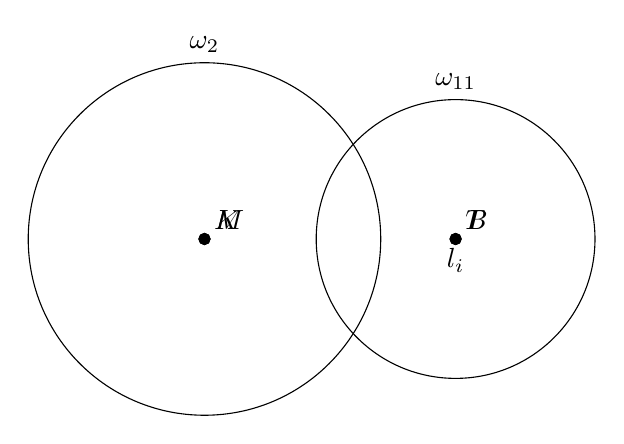
\begin{tikzpicture}[scale=1.0]
  \filldraw (0.0, 0.0) circle (2pt) node[above right] {$K$};
  \filldraw (0.0, 0.0) circle (2pt) node[above right] {$M$};
  \filldraw (3.1891, 0.0) circle (2pt) node[above right] {$B$};
  \filldraw (3.1891, 0.0) circle (2pt) node[above right] {$T$};
  \draw (3.1891, 0.0) -- (3.1891, 0.0) node[midway, below] {$l_i$};
  \draw (3.1891, 0.0) circle (1.7703) node[above=1.7703cm] {$\omega_{11}$};
  \draw (0.0, 0.0) circle (2.2384) node[above=2.2384cm] {$\omega_2$};
\end{tikzpicture}
\end{document}